\subsection{InternVL3-9B cross-backbone evaluation}
\label{app:internvl}

Figure~\ref{fig:internvl_trajectory} reports InternVL3-9B trajectories on VQA-RAD and MIMIC-CXR. The two tasks use independently trained models, with full-parameter supervised fine-tuning through LLaMA-Factory~\citep{zheng2024llamafactory}; each round continues from the preceding round's weights. The curves include the baseline and all eight completed training rounds.

VQA-RAD accuracy increases from 56.98\% to 77.38\% at round 8, a gain of 20.40 percentage points, and peaks at 78.71\% at round 6. MIMIC-CXR RaTEScore increases from 50.55 to 63.83, a gain of 13.28 points, with a maximum of 65.34 at round 4. The two trajectories reach their maxima at different stages and retain substantial gains at the final round.

\begin{figure}[H]
\centering
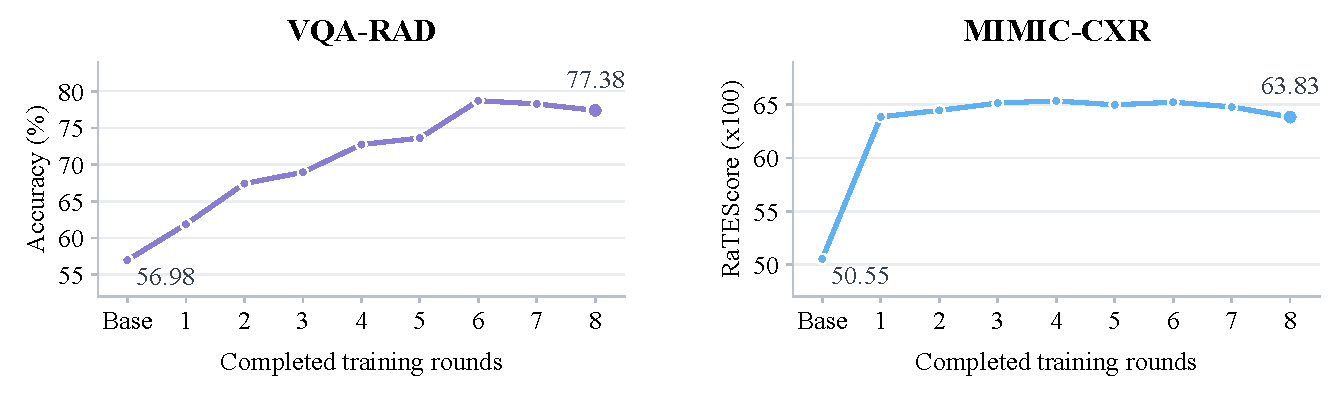
\includegraphics[width=\linewidth]{figures/internvl_trajectory.pdf}
\caption{InternVL3-9B learning trajectories. Left: VQA-RAD accuracy (\%). Right: MIMIC-CXR RaTEScore, scaled by 100. The panels correspond to independently trained task-specific models. Base denotes the initial model; rounds 1--8 denote completed training rounds. Only baseline and final values are annotated.}
\label{fig:internvl_trajectory}
\end{figure}
